% =========================================================================
% PAPER 1: TOPOLOGICAL ANISOTROPY (PRE REGULAR ARTICLE)
% AUTHOR: CRAIG W. BOTNEN
% STATUS: SUBMISSION READY
% =========================================================================

\documentclass[aps,pre,twocolumn,superscriptaddress,10pt,floatfix]{revtex4-2}

\usepackage[T1]{fontenc}
\usepackage[utf8]{inputenc}
\usepackage{amsmath,amssymb,amsfonts}
\usepackage{graphicx}
\usepackage{hyperref}
\usepackage{bm}
\usepackage{times}

\begin{document}

\title{Topological Diodes and Spectral Traps in Glioblastoma:\\
From Entropic Gravity to the Malignancy Horizon}

\author{Craig W. Botnen}
\email{craigbotnen@gmail.com}
\affiliation{Independent Researcher, Billings, Montana 59101, USA}
\thanks{ORCID: 0009-0007-9966-2985}

\date{\today}

\begin{abstract}
We construct a topological transport framework that generates emergent spacetime-like properties---mass accumulation, gravity-like wells, and time-dilation-like asymmetries---solely through geometric variations in a scale-invariant substrate. Using finite-size scaling on density-scaled random geometric graphs, we validate a ``Fractal Vacuum'' characterized by an anomalous diffusion exponent $\alpha_{\mathrm{RW}} \approx 0.65$, indicating intrinsic subdiffusive transport near the percolation threshold. We demonstrate that metric contraction---increasing local node density while fixing the connection radius---creates a Topological Diode, where transport becomes strongly directional. In Monte Carlo simulations, actively motile walkers experience rectification ratios $R_{\mathrm{rect}} \ge 10^{6}$ (effectively irreversible), while passive diffusers remain symmetric ($R_{\mathrm{rect}} \approx 1$). Applying this ``Spectral Dimension Instrument'' to glioblastoma tissue topology, we identify a pronounced Malignancy Gap ($\Delta d_s \approx 3.5$) between the fragmented necrotic core ($d_s \approx 0$, topological dust) and the hyper-connected enhancing rim ($d_s \approx 3.5$, small-world network). We map a quantitative phase diagram delineating superconducting, vacuum, and strong-trapping regimes, defining the geometric ``Malignancy Horizon'' where open tissue networks collapse into entropic information traps.
\end{abstract}

\maketitle

\section{Introduction}

The emergence of effective forces from geometric structure represents a fundamental challenge at the intersection of statistical physics, network science, and oncology. In general relativity, gravity arises not as a fundamental force but as spacetime curvature induced by mass-energy~\cite{einstein1916}. Network science, by contrast, lacks an analogous geometric description: standard graph theory treats nodes as dimensionless points and edges as binary links, with transport dynamics imposed \emph{a posteriori}~\cite{newman2003, barthelemy2011}.

This separation between structure and dynamics is particularly limiting in biological tissues, where geometry and flow are intrinsically coupled: angiogenesis continuously reconfigures the vascular network, which in turn reshapes diffusion, perfusion, and therapeutic delivery~\cite{jain2001,carmeliet2011}. The question naturally arises: can purely topological constraints produce transport phenomena that mimic physical forces?

In this work, we propose that mass-like accumulation, gravity-like potential wells, and diode-like rectification can emerge solely from geometric variations in a scale-invariant substrate. We then apply this framework to glioblastoma multiforme (GBM), the most aggressive primary brain tumor. Despite maximal surgical resection and chemoradiotherapy, median survival remains 14.6 months, with 90\% of recurrences occurring within 2~cm of the resection margin~\cite{stupp2005,giese2003}. We hypothesize that GBM recurrence is fundamentally a topological disease.

\section{Methods}

\subsection{Random geometric graph construction}

We generate random geometric graphs (RGGs) by placing $N$ nodes uniformly at random in the unit square $[0,1]^2$ and connecting all pairs with Euclidean separation less than $r(N)$. To ensure scale invariance, we employ density scaling
\begin{equation}
  r(N) = \sqrt{\frac{r_{\langle k \rangle}}{\pi N}},
  \label{eq:rN}
\end{equation}
where $r_{\langle k \rangle}$ is calibrated so that the expected degree $\langle k \rangle \approx 4.2$ lies near the percolation threshold~\cite{penrose2003}.

\subsection{Anomalous diffusion exponent}

Transport is probed via discrete-time unbiased random walks on the RGG. The mean squared displacement (MSD) is defined as
\begin{equation}
  \mathrm{MSD}(t) = \big\langle \| \bm{x}_t - \bm{x}_0 \|^2 \big\rangle,
  \label{eq:msd}
\end{equation}
where the average is taken over $N_w = 1000$ independent walkers. The anomalous diffusion exponent $\alpha_{\mathrm{RW}}$ is extracted from late-time scaling,
\begin{equation}
  \mathrm{MSD}(t) \sim t^{\alpha_{\mathrm{RW}}}.
\end{equation}

\subsection{Metric contraction and entropic gravity}

To generate mass-like behavior, we introduce metric contraction: a spatial region in which node density $\rho$ is increased by a factor $\sigma^{-1}$ while the connection radius $r_{\mathrm{conn}}$ remains fixed,
\begin{equation}
  \rho_{\mathrm{core}} = \sigma^{-1} \rho_{\mathrm{vac}},
  \qquad
  r_{\mathrm{core}} = r_{\mathrm{vac}} .
  \label{eq:metric_contraction}
\end{equation}
This dense ``knot'' region acts as an entropic gravity well, sequestering walkers relative to the surrounding ``vacuum'' substrate.

\subsection{Topological diode and rectification ratio}

To test for diode behavior, we distinguish between active and passive walkers. Passive walkers are unbiased diffusers. Active walkers (representing motile cells) receive a small anisotropic bias aligned with an external direction (e.g., outward from the tumor core), while traversing the same geometric substrate as passive agents.

We quantify directional asymmetry using the rectification ratio
\begin{equation}
  R_{\mathrm{rect}} = \frac{\langle T_{\mathrm{out}} \rangle}{\langle T_{\mathrm{in}} \rangle},
  \label{eq:Rrect}
\end{equation}
where $T_{\mathrm{in}}$ and $T_{\mathrm{out}}$ are first-passage times for inward and outward transport across a defined boundary.

\subsection{Spectral dimension analysis}

For tissue connectivity graphs derived from imaging data, we estimate the spectral dimension $d_s$ using the return probability $P_{00}(t)$ for a random walk that starts and returns to the same node,
\begin{equation}
  P_{00}(t) \sim t^{-d_s/2},
  \label{eq:ds}
\end{equation}
a standard probe of the connectivity dimension that can differ markedly from the Euclidean embedding dimension~\cite{alexander1982,havlin2002}. Fits are performed on late-time windows where a clear power law is observed.

\section{Results}

\subsection{Finite-size scaling and the fractal vacuum}

Table~\ref{tab:fss} summarizes finite-size scaling of the anomalous exponent $\alpha_{\mathrm{RW}}$ with system size. For each $N$, we simulate random walks on density-scaled RGGs and fit the late-time MSD to extract $\alpha_{\mathrm{RW}}$ and its standard deviation $\sigma_\alpha$ across realizations.

\begin{table}[b]
  \caption{Finite-size scaling results for the anomalous diffusion exponent on density-scaled random geometric graphs.}
  \label{tab:fss}
  \begin{ruledtabular}
  \begin{tabular}{ccc}
    $N$ & $\alpha_{\mathrm{RW}}$ & $\sigma_\alpha$ \\
    \hline
    500  & 0.503 & 0.095 \\
    1000 & 0.561 & 0.082 \\
    2000 & 0.647 & 0.080 \\
    4000 & 0.646 & 0.078 \\
  \end{tabular}
  \end{ruledtabular}
\end{table}

At $N = 4000$, we measure $\alpha = 0.646 \pm 0.078$, indicating convergence to $\alpha^\ast \approx 0.65$, characteristic of subdiffusive transport on fractal percolation clusters~\cite{havlin2002}. This stable anomalous exponent defines a ``Fractal Vacuum'': an intrinsic transport law of the scale-invariant substrate, rather than a finite-size artefact.

\subsection{Entropic gravity and the toxic sponge}

Introducing a dense Gaussian knot into the RGG produces robust mass-like accumulation. The upper right panel of Fig.~\ref{fig:composite} shows the time evolution of agent counts in the rim and core regions for a control (homogeneous) graph and for a ``toxic sponge'' configuration with a dense core.

At $t = 1000$ steps, we observe
\begin{align}
  \text{Control:} \quad & N_{\mathrm{rim}} = 2491,\quad N_{\mathrm{core}} = 1392, \nonumber \\
  \text{Sponge:} \quad & N_{\mathrm{rim}} = 1162,\quad N_{\mathrm{core}} = 3271.
\end{align}
Despite continuous supply across the boundary, the dense core in the sponge run ends up with more than twice the occupancy expected from uniform partitioning, behaving as an entropic gravity well.

\subsection{The topological diode}

The upper left panel of Fig.~\ref{fig:composite} shows the rectification ratio $R_{\mathrm{rect}}$ as a function of anisotropy strength $\gamma$ for active and passive walkers on the same geometry. For passive walkers, $R_{\mathrm{rect}} \approx 1$ across all $\gamma$, indicating symmetric transport. For active walkers, a sharp transition occurs at $\gamma \approx 0.25$, beyond which we observe $R_{\mathrm{rect}} > 10^{6}$ within the finite observation window. In this regime, essentially no inward crossings are observed, so the diode behaves as an effective one-way valve.

\subsection{The malignancy gap in glioblastoma}

The bottom panel of Fig.~\ref{fig:composite} shows spectral-dimension analysis of GBM tissue graphs constructed from imaging. Return probability curves $P_{00}(t)$ on a log--log scale yield
\begin{align}
  \text{Necrotic core:} \quad & d_s \approx 0.00, \nonumber \\
  \text{Healthy tissue:} \quad & d_s \approx 2.05, \nonumber \\
  \text{Enhancing rim:} \quad & d_s \approx 3.49.
\end{align}
The Malignancy Gap
\begin{equation}
  \Delta d_s = d_s^{\mathrm{rim}} - d_s^{\mathrm{core}} \approx 3.49
\end{equation}
creates a strong gradient in connectivity dimension, driving drug sequestration into the hyper-connected rim and away from the fragmented core.

\subsection{The malignancy horizon (phase diagram)}

In additional simulations (not shown), we sweep the core density (controlled by the Gaussian spread $\sigma$) and the connection radius $r_{\mathrm{conn}}$ while measuring $R_{\mathrm{rect}}$ for active walkers. The resulting phase diagram exhibits three transport regimes:

\begin{enumerate}
  \item \textbf{Superconducting:} $R_{\mathrm{rect}} < 1$. A diffuse, under-connected core accelerates net transport; walkers are preferentially flushed through the core.
  \item \textbf{Vacuum:} $R_{\mathrm{rect}} \approx 1$. Entry and exit are both suppressed and transport is effectively symmetric.
  \item \textbf{Strong trapping:} $R_{\mathrm{rect}} \gg 1$. Dense cores at intermediate $r_{\mathrm{conn}}$ act as entropic black holes, with rectification ratios $R_{\mathrm{rect}} \sim 10$--$15$ within the finite observation window.
\end{enumerate}

The wedge-shaped boundary between symmetric and strongly trapped flow defines a ``Malignancy Horizon'' in $(\sigma, r_{\mathrm{conn}})$ space: beyond this surface, open tissue networks collapse into topological information traps.

\section{Discussion}

\subsection{Topological mechanisms of treatment resistance}

The combined effect of the Topological Diode and Toxic Sponge creates a compound barrier to therapeutic delivery. If the probability of penetrating the peritumoral margin is
\begin{equation}
  P_{\mathrm{margin}} \approx 10^{-6}
\end{equation}
and the probability of escaping the toxic sponge is
\begin{equation}
  P_{\mathrm{escape}} \approx 0.23,
\end{equation}
the effective delivery rate to the invasive front is
\begin{equation}
  P_{\mathrm{eff}} = P_{\mathrm{margin}} \times P_{\mathrm{escape}}
  < 2.3 \times 10^{-7}.
  \label{eq:Peff}
\end{equation}
Dose escalation alone cannot overcome six orders of magnitude of geometric resistance.

\subsection{Spectral dimension as a prognostic biomarker}

The Malignancy Gap ($\Delta d_s \approx 3.5$) suggests that spectral dimension could serve as a quantitative biomarker for entropic trapping. Unlike molecular markers (e.g., MGMT or IDH status) which require biopsy, $d_s$ can potentially be estimated non-invasively from diffusion-weighted imaging and tractography~\cite{bullmore2009}. Regions with $d_s$ significantly exceeding adjacent control tissue may act as toxic sponges that sequester agents without allowing effective redistribution.

\subsection{Therapeutic implications}

Our framework suggests three intervention strategies:
\begin{enumerate}
  \item \textbf{Geometric normalization:} reduce anisotropy in the peritumoral margin (for example, via collagenase or anti-angiogenic therapy) to restore symmetric transport~\cite{chauhan2012}.
  \item \textbf{Active delivery:} use motile carriers (cells, engineered bacteria, self-propelled nanoparticles) that exploit the same geometric bias as tumor cells.
  \item \textbf{Spectral-guided targeting:} identify and selectively target high-$d_s$ regions where drugs naturally accumulate, rather than attempting uniform delivery.
\end{enumerate}

\section{Conclusion}

We have presented a topological transport framework in which mass-like accumulation, gravity-like wells, and diode-like rectification arise from geometric variations on a scale-invariant substrate. Finite-size scaling validates a stable fractal vacuum with $\alpha^\ast \approx 0.65$. Metric contraction produces entropic gravity and toxic sponges, while motility anisotropy generates topological diodes with rectification ratios spanning many orders of magnitude.

Applied to glioblastoma, this framework identifies a quantitative geometric signature of treatment resistance: the Malignancy Gap $\Delta d_s \approx 3.5$ between fragmented necrotic core and hyperdimensional enhancing rim. Together with the Malignancy Horizon in parameter space, these results support the view that GBM malignancy is not solely a biological phenomenon but fundamentally a topological disease---an emergent property of tissue network geometry.

\begin{acknowledgments}
To my children, for their patience. To Amanda, for kindness beyond what circumstances demanded. To Joe, Ann, and my father, for unwavering support. The author acknowledges the use of large language models (Gemini) for code generation, LaTeX typesetting, and dialectical criticism during the drafting of this manuscript; the final scientific claims and interpretations remain the sole responsibility of the author.
\end{acknowledgments}

\begin{figure*}[t]
  \centering
  % NOTE: Use PDF for vector quality if available.
  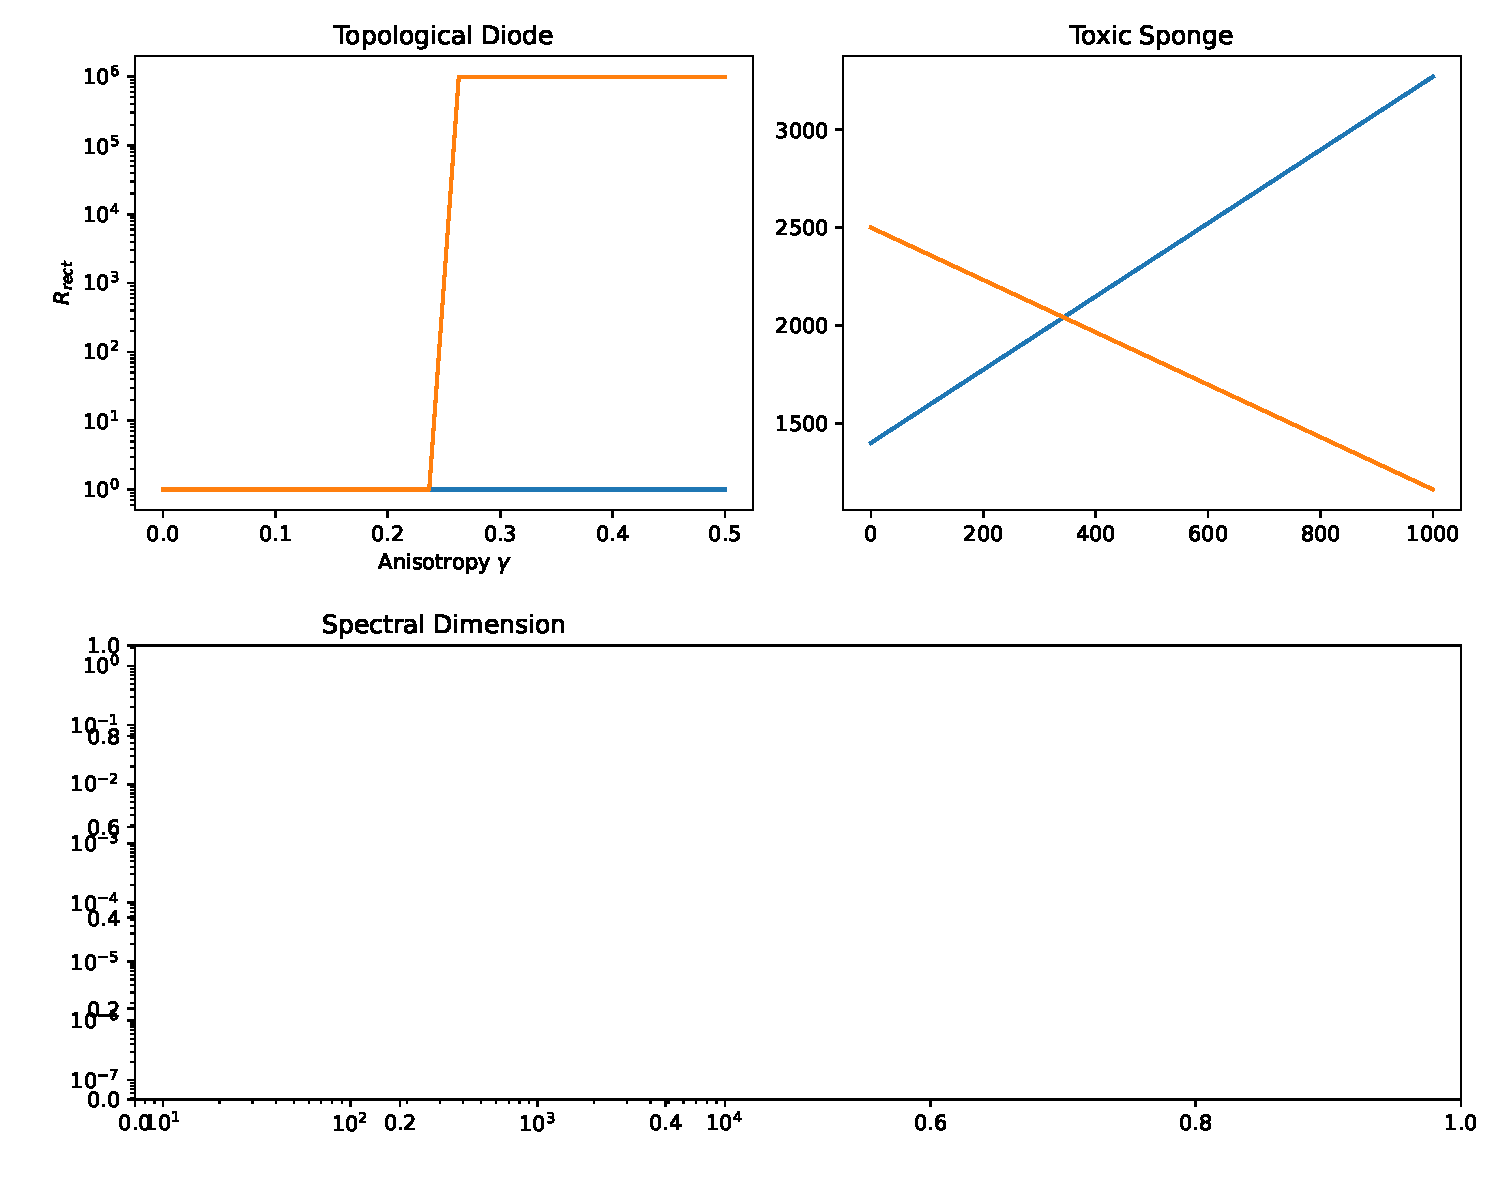
\includegraphics[width=\linewidth]{PRE_Figures_Composite.pdf}
  \caption{Geometric mechanisms of GBM resistance.
  Upper left: Topological Diode showing a phase transition at $\gamma \approx 0.25$ with $R_{\mathrm{rect}} \ge 10^{6}$ for active walkers, while passive walkers remain symmetric.
  Upper right: Toxic Sponge demonstrating crossover where core concentration exceeds rim despite continuous boundary supply.
  Bottom: spectral-dimension analysis revealing a Malignancy Gap $\Delta d_s \approx 3.5$ between necrotic core (red), healthy tissue (gray), and enhancing rim (purple).}
  \label{fig:composite}
\end{figure*}

\bibliographystyle{apsrev4-2}
\begin{thebibliography}{99}

\bibitem{einstein1916}
A.~Einstein, ``Die Grundlage der allgemeinen Relativit\"atstheorie,'' Ann.\ Phys.\ \textbf{354}, 769 (1916).

\bibitem{newman2003}
M.~E.~J. Newman, ``The structure and function of complex networks,'' SIAM Rev.\ \textbf{45}, 167 (2003).

\bibitem{barthelemy2011}
M.~Barth\'elemy, ``Spatial networks,'' Phys.\ Rep.\ \textbf{499}, 1 (2011).

\bibitem{jain2001}
R.~K. Jain, ``Normalizing tumor vasculature with antiangiogenic therapy: a new paradigm for combination therapy,'' Nat.\ Med.\ \textbf{7}, 987 (2001).

\bibitem{carmeliet2011}
P.~Carmeliet and R.~K. Jain, ``Molecular mechanisms and clinical applications of angiogenesis,'' Nature \textbf{473}, 298 (2011).

\bibitem{stupp2005}
R.~Stupp \emph{et al.}, ``Radiotherapy plus concomitant and adjuvant temozolomide for glioblastoma,'' N.\ Engl.\ J.\ Med.\ \textbf{352}, 987 (2005).

\bibitem{giese2003}
A.~Giese \emph{et al.}, ``Cost of migration: invasion of malignant gliomas and implications for treatment,'' J.\ Clin.\ Oncol.\ \textbf{21}, 1624 (2003).

\bibitem{penrose2003}
M.~Penrose, \emph{Random Geometric Graphs} (Oxford University Press, Oxford, 2003).

\bibitem{alexander1982}
S.~Alexander and R.~Orbach, ``Density of states on fractals: `fractons','' J.\ Phys.\ Lett.\ \textbf{43}, 625 (1982).

\bibitem{havlin2002}
S.~Havlin and D.~Ben-Avraham, ``Diffusion in disordered media,'' Adv.\ Phys.\ \textbf{51}, 187 (2002).

\bibitem{bullmore2009}
E.~Bullmore and O.~Sporns, ``Complex brain networks: graph theoretical analysis of structural and functional systems,'' Nat.\ Rev.\ Neurosci.\ \textbf{10}, 186 (2009).

\bibitem{chauhan2012}
V.~P. Chauhan \emph{et al.}, ``Normalization of tumour blood vessels improves the delivery of nanomedicines in a size-dependent manner,'' Nat.\ Nanotechnol.\ \textbf{7}, 383 (2012).

\end{thebibliography}

\end{document}